\documentclass[11pt,a4paper]{article}

\usepackage[utf8]{inputenc}
\usepackage[T1]{fontenc}
\usepackage{mathpazo}
\usepackage[scaled=0.92]{helvet}
\usepackage[margin=1in]{geometry}
\usepackage{graphicx}
\usepackage{amsmath,amssymb,amsfonts}
\usepackage{booktabs}
\usepackage{tabularx}
\usepackage{setspace}
\usepackage{titlesec}
\usepackage{fancyhdr}
\usepackage{float}
\usepackage{caption}

\usepackage{tikz}
\usetikzlibrary{shapes.geometric, arrows.meta, positioning, calc, shadows, backgrounds}
\usepackage[hidelinks]{hyperref}

\setstretch{1.15}
\setlength{\parindent}{0pt}
\setlength{\parskip}{8pt}
\sloppy

\titleformat{\section}{\normalfont\large\bfseries\sffamily}{\thesection}{1em}{}
\titleformat{\subsection}{\normalfont\normalsize\bfseries\sffamily}{\thesubsection}{1em}{}

\pagestyle{fancy}
\fancyhf{}
\fancyhead[L]{\small\sffamily Analisis Pemodelan Data Lanjutan: EER Diagram}
\fancyhead[R]{\small\sffamily\thepage}
\renewcommand{\headrulewidth}{0.4pt}

\captionsetup{font=small,labelfont=bf,labelsep=period}

\renewenvironment{abstract}
{\small
	\begin{center}\textbf{\sffamily Abstract}\end{center}
	\begin{quote}}
	{\end{quote}}

\title{\vspace{-1.5cm}\textbf{\sffamily\LARGE Analisis Pemodelan Data Lanjutan: \\ Enhanced Entity Relationship Diagram (EERD)}}
\author{
	\textbf{Muhammad Riduwan Khafidi} \\
	\small Program Studi Teknik Rekayasa Perangkat Lunak \\
	\small Politeknik Negeri Batam \\
	\small \texttt{4342611034@students.polibatam.ac.id}
}
\date{\small\today}

\begin{document}

\maketitle
\thispagestyle{empty}

\begin{abstract}
	Entity Relationship Diagram (ERD) standar terkadang tidak cukup untuk merepresentasikan kompleksitas aturan bisnis di dunia nyata. Untuk mengatasi keterbatasan ini, muncullah Enhanced Entity Relationship Diagram (EERD). EERD memperluas konsep ERD dengan menambahkan fitur-fitur berorientasi objek seperti Spesialisasi (Specialization), Generalisasi (Generalization), Pewarisan (Inheritance), dan Agregasi (Aggregation). Makalah ini membedah secara komprehensif mekanisme EERD dalam memodelkan hirarki entitas, di mana sebuah entitas induk dapat memiliki sub-entitas yang lebih spesifik. Melalui visualisasi diagram, makalah ini menjelaskan bagaimana atribut dan relasi diwariskan dari entitas tingkat tinggi ke tingkat rendah, serta bagaimana sebuah relasi dapat diabstraksikan menjadi entitas baru (agregasi) untuk memenuhi aturan temporal (waktu) dalam suatu transaksi.
\end{abstract}

\section{Pendahuluan: Mengapa ERD Perlu Diperluas?}

Dalam praktikum sebelumnya, kita telah memahami bahwa ERD adalah fondasi untuk memetakan entitas dan relasi. Namun, bayangkan sebuah universitas yang memiliki dua jenis dosen: Dosen Tetap (Permanent Lecturer) dan Dosen Tidak Tetap (Part-time Lecturer). Kedua jenis dosen ini memiliki atribut yang sama seperti Nama, ID Pegawai, dan Alamat. Namun, Dosen Tetap memiliki atribut spesifik seperti Golongan (Grade) dan Tanggal Mulai, sedangkan Dosen Tidak Tetap memiliki atribut seperti Nama Perusahaan dan Jumlah Jam Mengajar.

Jika kita memaksakan keduanya ke dalam satu entitas "Dosen", akan banyak atribut yang kosong (bernilai \textit{null}). Jika kita memisahkannya menjadi dua entitas yang benar-benar terpisah, kita akan kehilangan esensi bahwa keduanya sama-sama "Dosen". Di sinilah Enhanced Entity Relationship Diagram (EERD) hadir sebagai solusi. EERD memungkinkan kita merancang sub-kelompok dari sebuah entitas set, sebuah konsep yang disebut Spesialisasi.

\section{Spesialisasi (Specialization)}

Spesialisasi adalah proses desain untuk membuat sub-kelompok (sub-entitas) dari sebuah entitas set berdasarkan karakteristik atau atribut yang berbeda. Ini adalah pendekatan \textit{top-down}, di mana kita memulai dari entitas yang paling umum (Superclass), lalu memecahnya menjadi entitas yang lebih spesifik (Subclass).

Dalam notasi EERD, Spesialisasi digambarkan dengan sebuah segitiga terbalik yang di dalamnya terdapat tulisan \textbf{IS A} (adalah sebuah). Segitiga ini menghubungkan Superclass di atas dengan Subclass di bawahnya. Perhatikan Gambar \ref{fig:specialization} di bawah ini.

\begin{figure}[H]
	\centering
	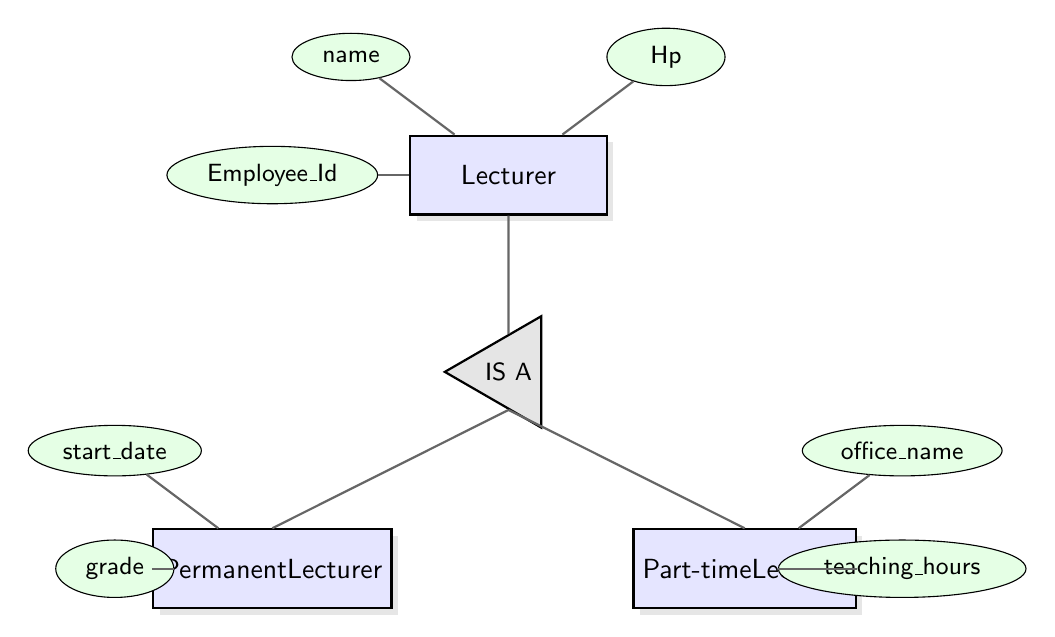
\begin{tikzpicture}[
			entity/.style={draw, rectangle, minimum width=2.5cm, minimum height=1cm, fill=blue!10, thick, font=\sffamily, drop shadow={opacity=0.2}},
			attr/.style={draw, ellipse, minimum width=1.5cm, minimum height=0.6cm, fill=green!10, font=\small\sffamily},
			isa/.style={draw, isosceles triangle, isosceles triangle apex angle=60, shape border rotate=180, fill=gray!20, thick, font=\sffamily\small},
			line/.style={thick, color=gray!80!black}
		]
		% Superclass
		\node[entity] (lecturer) at (0,0) {Lecturer};
		\node[attr] (id) at (-3,0) {Employee\_Id};
		\node[attr] (name) at (-2,1.5) {name};
		\node[attr] (hp) at (2,1.5) {Hp};
		\draw[line] (lecturer) -- (id);
		\draw[line] (lecturer) -- (name);
		\draw[line] (lecturer) -- (hp);

		% IS A Triangle
		\node[isa] (is_a) at (0,-2.5) {IS A};
		\draw[line] (lecturer) -- (is_a);

		% Subclasses
		\node[entity] (perm) at (-3,-5) {Permanent\\Lecturer};
		\node[entity] (part) at (3,-5) {Part-time\\Lecturer};
		\draw[line] (is_a.south) -- (perm.north);
		\draw[line] (is_a.south) -- (part.north);

		% Subclass Attributes
		\node[attr] (grade) at (-5,-5) {grade};
		\node[attr] (start) at (-5,-3.5) {start\_date};
		\draw[line] (perm) -- (grade);
		\draw[line] (perm) -- (start);

		\node[attr] (office) at (5,-3.5) {office\_name};
		\node[attr] (hours) at (5,-5) {teaching\_hours};
		\draw[line] (part) -- (office);
		\draw[line] (part) -- (hours);
	\end{tikzpicture}
	\caption{Contoh Spesialisasi pada Entitas Lecturer.}
	\label{fig:specialization}
\end{figure}

Melalui Spesialisasi, entitas "Permanent Lecturer" hanya akan memiliki atribut spesifiknya sendiri tanpa harus memaksakan atribut "Part-time Lecturer" masuk ke dalamnya.

\section{Generalisasi (Generalization)}

Jika Spesialisasi adalah pendekatan \textit{top-down}, maka Generalisasi adalah kebalikannya, yaitu pendekatan \textit{bottom-up}. Generalisasi adalah proses menggabungkan beberapa entitas set yang memiliki atribut serupa menjadi satu entitas set yang lebih umum (Superclass).

Sebagai contoh, bayangkan kita memiliki entitas "Mahasiswa D3" dan "Mahasiswa D4". Setelah dianalisis, ternyata keduanya memiliki atribut yang sama persis (NIM, Nama, Jurusan, IPK), kecuali pada jenjang pendidikannya. Daripada membuat dua tabel terpisah, kita dapat menggeneralisasi keduanya menjadi satu entitas "Mahasiswa", lalu menambahkan satu atribut baru untuk menyimpan status jenjang (D3 atau D4), seperti yang diilustrasikan pada Gambar \ref{fig:generalization}.

\begin{figure}[H]
	\centering
	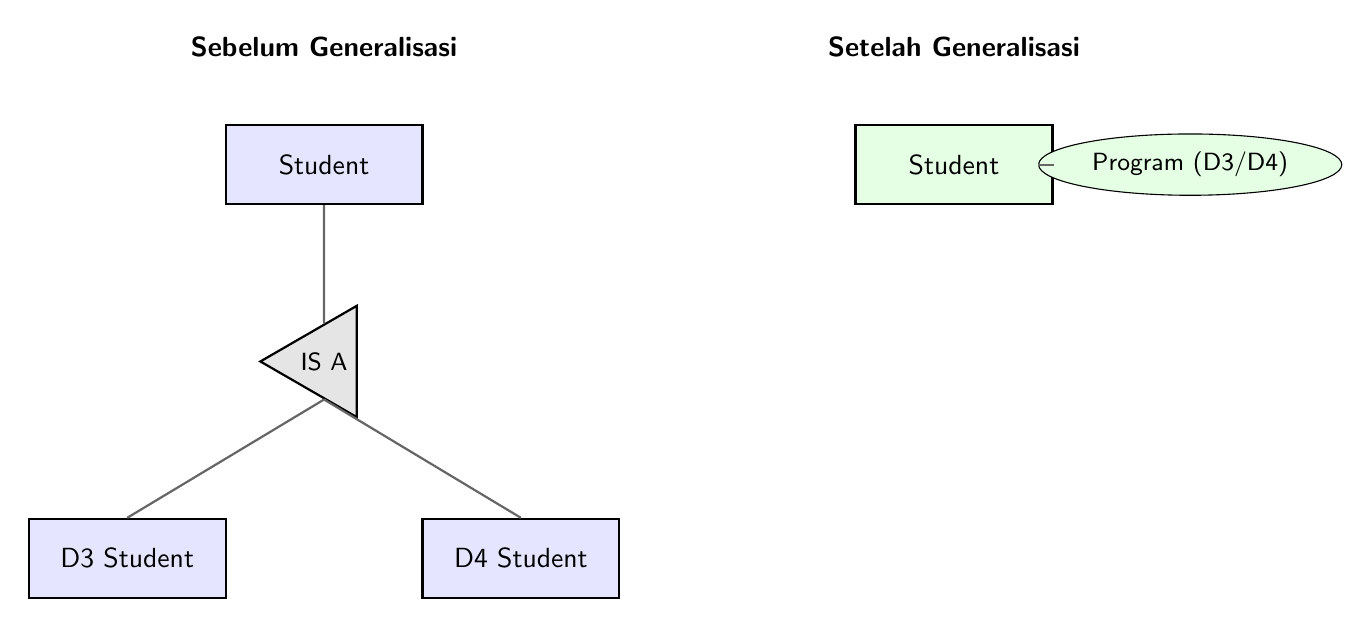
\begin{tikzpicture}[
			entity/.style={draw, rectangle, minimum width=2.5cm, minimum height=1cm, fill=blue!10, thick, font=\sffamily},
			isa/.style={draw, isosceles triangle, isosceles triangle apex angle=60, shape border rotate=180, fill=gray!20, thick, font=\sffamily\small},
			line/.style={thick, color=gray!80!black}
		]
		% Before
		\node[font=\bfseries\sffamily] at (0,3) {Sebelum Generalisasi};
		\node[entity] (student) at (0,1.5) {Student};
		\node[isa] (is_a) at (0,-1) {IS A};
		\draw[line] (student) -- (is_a);
		\node[entity] (d3) at (-2.5,-3.5) {D3 Student};
		\node[entity] (d4) at (2.5,-3.5) {D4 Student};
		\draw[line] (is_a.south) -- (d3.north);
		\draw[line] (is_a.south) -- (d4.north);

		% After
		\node[font=\bfseries\sffamily] at (8,3) {Setelah Generalisasi};
		\node[entity, fill=green!10] (student_after) at (8,1.5) {Student};
		\node[draw, ellipse, fill=green!10, font=\small\sffamily] (prog) at (11,1.5) {Program (D3/D4)};
		\draw[line] (student_after) -- (prog);
	\end{tikzpicture}
	\caption{Proses Generalisasi Entitas Mahasiswa.}
	\label{fig:generalization}
\end{figure}

\section{Pewarisan (Inheritance)}

Konsep kunci dalam EERD adalah \textbf{Pewarisan} (\textit{Inheritance}). Sebuah sub-entitas secara otomatis mewarisi seluruh atribut dan relasi yang dimiliki oleh entitas induknya (Superclass).

Sebagai contoh, karena "Permanent Lecturer" adalah bagian dari "Lecturer", maka ia otomatis memiliki atribut \textit{Employee\_Id}, \textit{name}, dan \textit{Hp} tanpa perlu mendeklarasikannya ulang. Selain atribut, relasi juga diwariskan. Jika entitas "Lecturer" memiliki relasi "mengajar" (teach) ke entitas "Student", maka baik "Permanent Lecturer" maupun "Part-time Lecturer" juga memiliki relasi tersebut. Namun, sub-entitas juga diizinkan untuk memiliki relasi eksklusif yang tidak dimiliki oleh sub-entitas lainnya, seperti yang ditunjukkan pada Gambar \ref{fig:rel_inheritance}.

\begin{figure}[H]
	\centering
	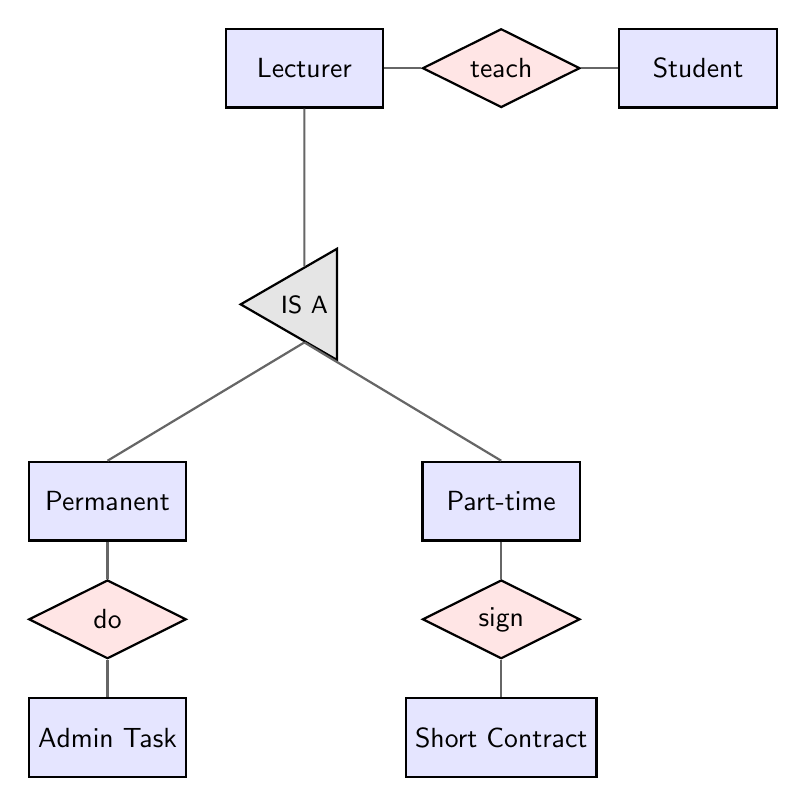
\begin{tikzpicture}[
			entity/.style={draw, rectangle, minimum width=2cm, minimum height=1cm, fill=blue!10, thick, font=\sffamily},
			rel/.style={draw, diamond, aspect=2, minimum width=2cm, minimum height=1cm, fill=red!10, thick, font=\sffamily},
			isa/.style={draw, isosceles triangle, isosceles triangle apex angle=60, shape border rotate=180, fill=gray!20, thick, font=\sffamily\small},
			line/.style={thick, color=gray!80!black}
		]
		\node[entity] (lecturer) at (0,2) {Lecturer};
		\node[entity] (student) at (5,2) {Student};
		\node[rel] (teach) at (2.5,2) {teach};
		\draw[line] (lecturer) -- (teach);
		\draw[line] (teach) -- (student);

		\node[isa] (is_a) at (0,-1) {IS A};
		\draw[line] (lecturer) -- (is_a);

		\node[entity] (perm) at (-2.5,-3.5) {Permanent};
		\node[entity] (part) at (2.5,-3.5) {Part-time};
		\draw[line] (is_a.south) -- (perm.north);
		\draw[line] (is_a.south) -- (part.north);

		\node[entity] (admin) at (-2.5,-6.5) {Admin Task};
		\node[rel] (do) at (-2.5,-5) {do};
		\draw[line] (perm) -- (do);
		\draw[line] (do) -- (admin);

		\node[entity] (contract) at (2.5,-6.5) {Short Contract};
		\node[rel] (sign) at (2.5,-5) {sign};
		\draw[line] (part) -- (sign);
		\draw[line] (sign) -- (contract);
	\end{tikzpicture}
	\caption{Pewarisan Relasi dan Relasi Eksklusif pada Sub-entitas.}
	\label{fig:rel_inheritance}
\end{figure}

\section{Agregasi (Aggregation)}

Dalam pemodelan bisnis nyata, terkadang kita menjumpai sebuah relasi yang baru bisa terjadi \textit{setelah} relasi lainnya terjadi. Sebagai contoh, pada sistem perbankan, seorang "Customer" meminjam uang (relasi \textit{borrow}) ke entitas "Loan". Setelah pinjaman itu terjadi, barulah muncul transaksi "Pembayaran" (relasi \textit{pay}) ke entitas "Payment".

Kita tidak bisa langsung menghubungkan entitas "Payment" ke entitas "Customer" atau "Loan" secara langsung, karena pembayaran hanya valid jika ada pinjaman. Untuk merepresentasikan hal ini, kita menggunakan konsep \textbf{Agregasi}. Agregasi adalah abstraksi di mana sebuah relasi (beserta entitas-entitas yang terlibat di dalamnya) diperlakukan sebagai satu entitas set baru (entitas tingkat tinggi).

Perhatikan perbedaan desain pada Gambar \ref{fig:aggregation}.

\begin{figure}[H]
	\centering
	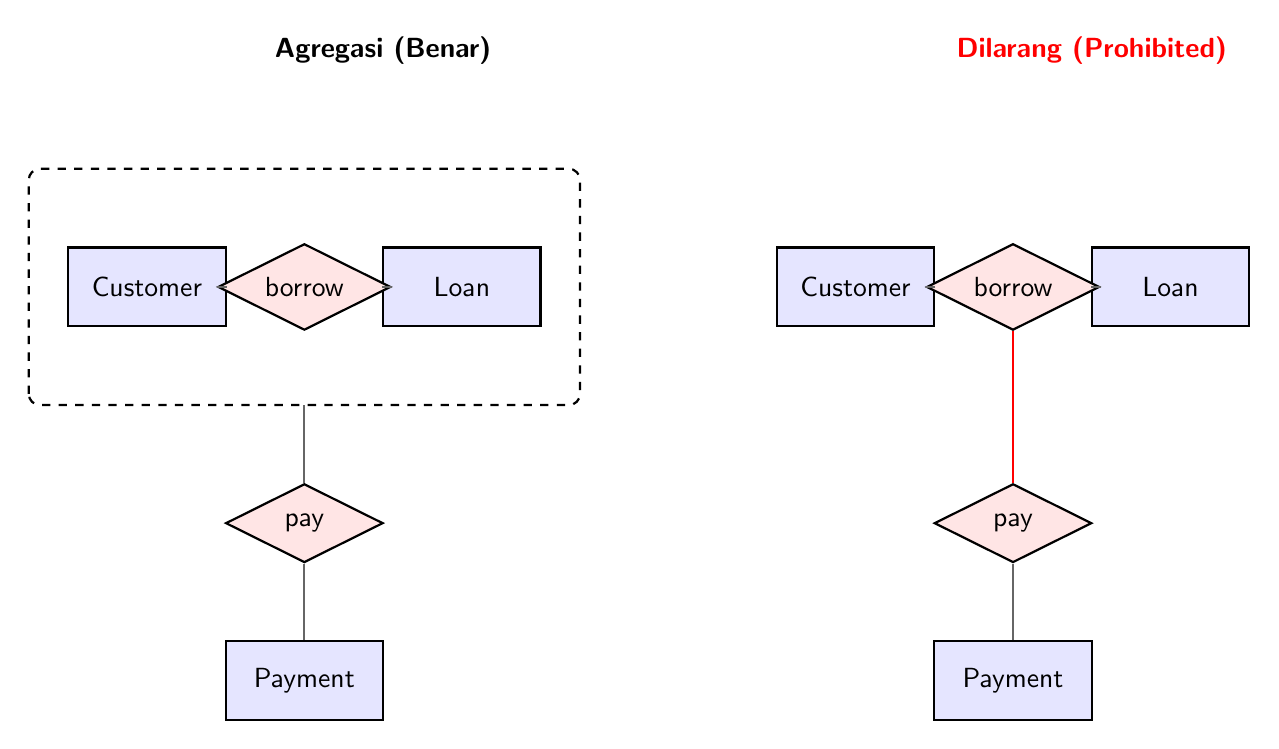
\begin{tikzpicture}[
			entity/.style={draw, rectangle, minimum width=2cm, minimum height=1cm, fill=blue!10, thick, font=\sffamily},
			rel/.style={draw, diamond, aspect=2, minimum width=2cm, minimum height=1cm, fill=red!10, thick, font=\sffamily},
			line/.style={thick, color=gray!80!black}
		]
		% Model Agregasi yang Benar
		\begin{scope}[shift={(0,0)}]
			\node[font=\bfseries\sffamily] at (3,3) {Agregasi (Benar)};
			\draw[dashed, thick, rounded corners] (-1.5,-1.5) rectangle (5.5,1.5);

			\node[entity] (cust) at (0,0) {Customer};
			\node[entity] (loan) at (4,0) {Loan};
			\node[rel] (borrow) at (2,0) {borrow};
			\draw[line] (cust) -- (borrow);
			\draw[line] (borrow) -- (loan);

			\node[rel] (pay) at (2,-3) {pay};
			\node[entity] (payment) at (2,-5) {Payment};

			\draw[line] (2,-1.5) -- (pay);
			\draw[line] (pay) -- (payment);
		\end{scope}

		% Model Salah (Prohibited)
		\begin{scope}[shift={(9,0)}]
			\node[font=\bfseries\sffamily, text=red] at (3,3) {Dilarang (Prohibited)};
			\node[entity] (cust2) at (0,0) {Customer};
			\node[entity] (loan2) at (4,0) {Loan};
			\node[rel] (borrow2) at (2,0) {borrow};
			\draw[line] (cust2) -- (borrow2);
			\draw[line] (borrow2) -- (loan2);

			\node[rel] (pay2) at (2,-3) {pay};
			\node[entity] (payment2) at (2,-5) {Payment};

			\draw[line, red] (borrow2) -- (pay2);
			\draw[line] (pay2) -- (payment2);
		\end{scope}
	\end{tikzpicture}
	\caption{Representasi Agregasi pada Relasi Pinjaman dan Pembayaran.}
	\label{fig:aggregation}
\end{figure}

Pada gambar di atas, kotak bergaris putus-putus menandakan bahwa "Customer", "Loan", dan relasi "borrow" telah diagregasi menjadi satu kesatuan entitas. Dengan demikian, relasi "pay" dapat dihubungkan ke agregat tersebut. Menghubungkan relasi secara langsung ke relasi lain (seperti pada gambar kanan) adalah hal yang dilarang dalam aturan baku EERD.

\section{Kesimpulan}

Enhanced Entity Relationship Diagram (EERD) memberikan kekuatan lebih bagi perancang basis data untuk memodelkan aturan bisnis yang kompleks. Melalui Spesialisasi dan Generalisasi, kita dapat mengelola hirarki entitas secara efisien, memastikan bahwa setiap entitas hanya menyimpan atribut yang relevan tanpa terjadi duplikasi. Konsep Pewarisan (Inheritance) memudahkan pemeliharaan relasi antar entitas. Sementara itu, Agregasi memungkinkan kita memodelkan ketergantungan temporal antar relasi, di mana sebuah transaksi baru dapat terjadi setelah transaksi sebelumnya tervalidasi. Penguasaan EERD adalah jembatan krusial sebelum skema konseptual ini ditransformasikan menjadi tabel fisik yang dinormalisasi di dalam DBMS.

\newpage
\section*{Referensi}
\addcontentsline{toc}{section}{Referensi}

\begin{thebibliography}{99}
	\bibitem{lubis}
	Lubis, A. I. (2026). \textit{Enhanced Entity Relationship Diagram} [Slide Presentasi Mata Kuliah Pengantar Basis Data]. Politeknik Negeri Batam.

	\bibitem{silberschatz}
	Silberschatz, A., Korth, H. F., \& Sudarshan, S. (2019). \textit{Database System Concepts} (7th ed.). McGraw-Hill Education.

	\bibitem{fathan}
	Fathan, S. (2012). \textit{Basis Data Edisi Revisi}. Penerbit Informatika.

	\bibitem{kadir}
	Kadir, A. (2009). \textit{Dasar Perancangan dan Implementasi Database Relasional}. Penerbit Andi.
\end{thebibliography}

\end{document}
